\section{Problem 4}

\subsection{Question}
\vspace*{10pt}
Determine if the friendship paradox holds for your Twitter account.
Since Twitter is a directed graph, use \enquote{followers} as value you measure 
$($i.e., \enquote{do your followers have more followers than you?}$)$.\\
\\
Generate the same graph as in question \#1, and calcuate the same 
mean, standard deviation, and median values.\\
\\
For the Twitter 1.1 API to help gather this data, see:
\\
\url{https://dev.twitter.com/docs/api/1.1/get/followers/list}
\\
If you do not have followers on Twitter (or don't have more than 50),
then use my twitter account \enquote{phonedude\_mln}.

\subsection{Answer}
Same instructions explained in question 2 are used to answer this question. As I remember, only one change has been made to {\it qet\_followers.py}. 
\\
\begin{itemize}
\item The old request:
\lstinputlisting[language=Python, linerange={73-73},stepnumber=0, caption={get\_followers.py}, label=listing:get_followers1]{q2/get_followers.py}
\item After modifying:
\lstinputlisting[language=Python,linerange={73-73},stepnumber=0, caption={get\_friends.py}, label=listing:get_friends]{q4/get_friends.py}
\end{itemize}
All new changes are stored in a new file called {\it qet\_friends.py}. The following is the output after running the Python program:
\vspace{2mm}
\begin{figure}[h!]
\centering
\fbox{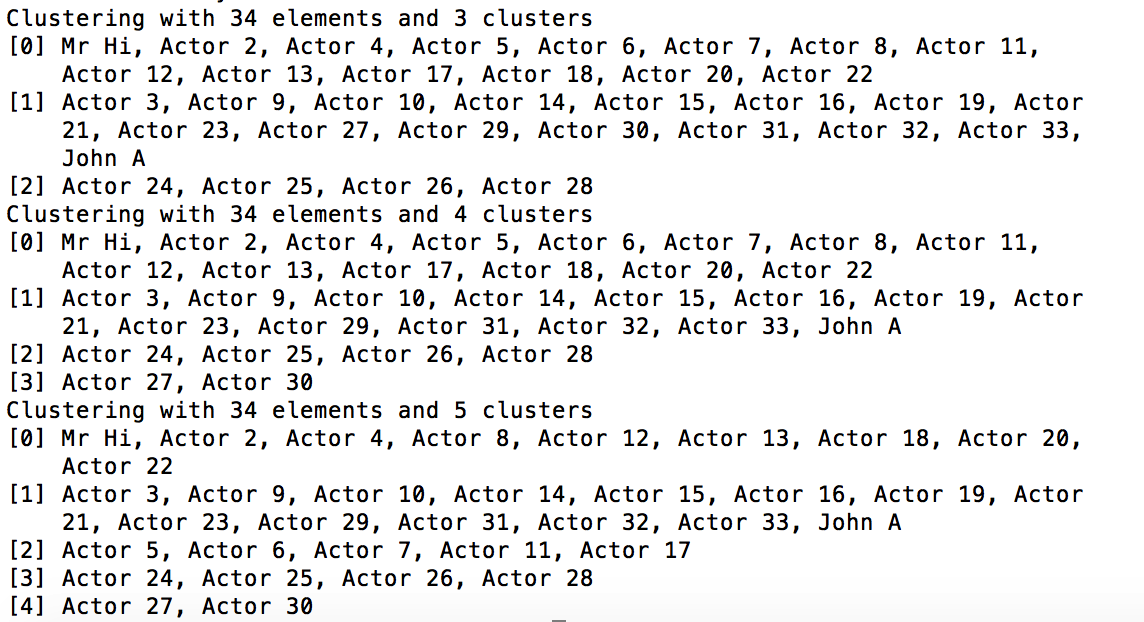
\includegraphics[scale=0.65]{q4/fig3.png}}
\caption{Sample output of number of following}
\label{fig:number_following}
\end{figure}
\newpage
\vspace*{2mm}
\begin{table}
\centering
\begin{tabular}{ l l }
\hline
\textbf{Mean} & 484.9214 \\
\textbf{Median} & 225 \\
\textbf{Std Dev} & 729.5275\\
\hline
\end{tabular}
\caption{Statistics on the count of Dr.Nelson Following, values straight from R}
\label{tab:q4stats}
\end{table}
\begin{figure}[h!]
\centering
\fbox{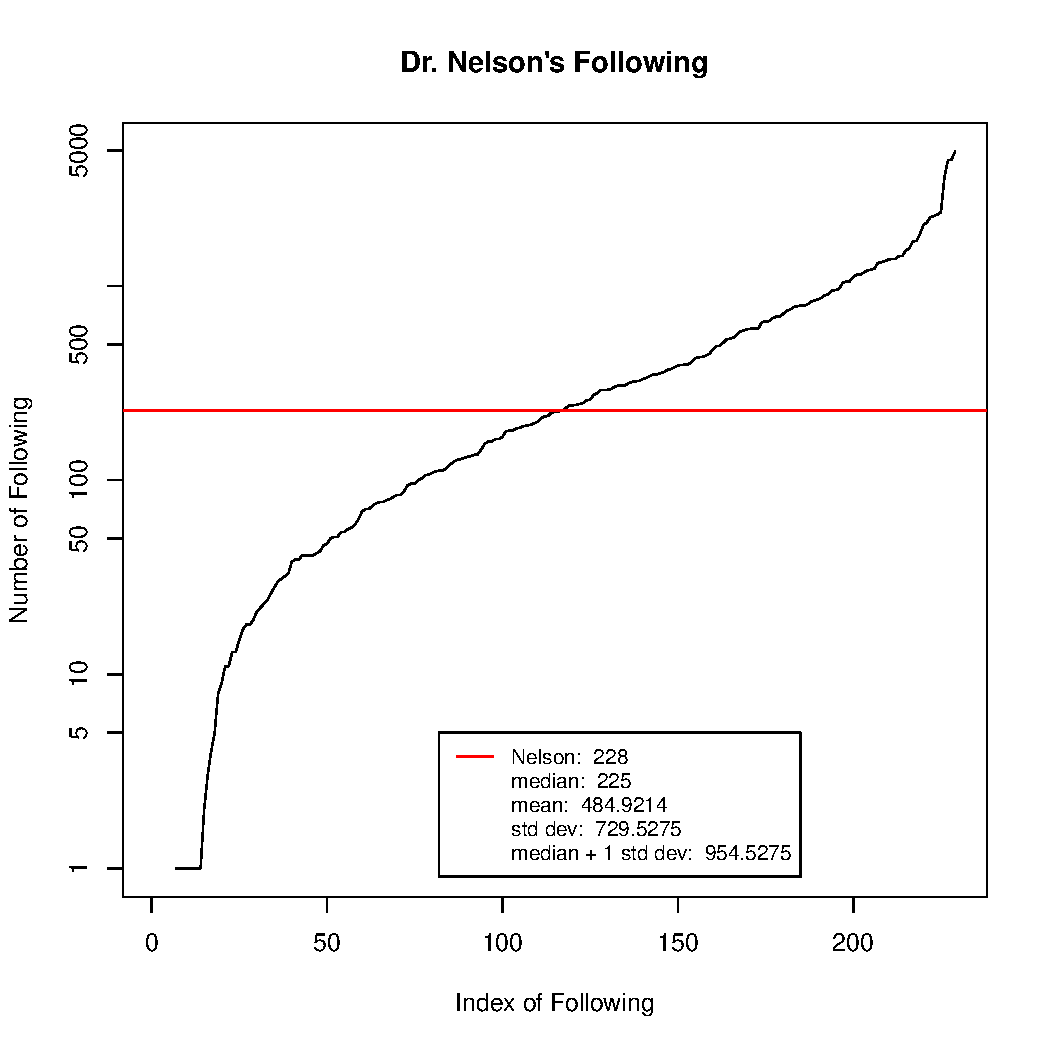
\includegraphics[scale=0.75]{q4/friend_plot.pdf}}
\caption{The Friendship Graph for Twitter Following}
\label{fig:followings_graph}
\end{figure}

I think here also the friendship paradox holds for Dr. Nelson Twitter account (for following) since the mean is equal to 484.9214 which greater than most of the number of following of Dr. Nelson following including himself. 